\documentclass[11pt,a4paper]{article}

% ------------------------------------------------------------------ à compléter
\newcommand{\etudiantA}{Taha Bachir El Bouhali}
\newcommand{\etudiantB}{Hsain Zaid}
\newcommand{\encadrant}{Pr. Abderrahim Elqadi}
\newcommand{\etablissement}{ENSAM Rabat}
\def\formation{}  % filière / module ; laissé vide, rien n'est affiché
\newcommand{\annee}{Année universitaire 2026--2027}

% ------------------------------------------------------------------ paquets
\usepackage[utf8]{inputenc}
\usepackage[T1]{fontenc}
\usepackage[french]{babel}
\frenchsetup{StandardItemLabels=true}
\usepackage{lmodern}
\usepackage{microtype}
\usepackage[a4paper,margin=2.2cm,top=2.3cm,bottom=2.3cm]{geometry}
\usepackage{graphicx}
\usepackage{booktabs}
\usepackage{tabularx}
\usepackage{float}
\usepackage{caption}
\usepackage{subcaption}
\usepackage{xcolor}
\usepackage{enumitem}
\usepackage{csquotes}
\usepackage{fancyhdr}
\usepackage{titlesec}
\usepackage{tikz}
\usetikzlibrary{arrows.meta,positioning,calc}
\usepackage[hidelinks]{hyperref}

% Fichier généré par make_figures.py à partir des résultats du benchmark. Ne pas modifier à la main.
\newcommand{\nMaxTrain}{2\,140\,000}
\newcommand{\nMilleTrain}{1\,070\,000}
\newcommand{\nUnTrain}{1\,070}
\newcommand{\scaleMax}{2000}
\newcommand{\skFitLRMax}{7{,}79}
\newcommand{\spFitLRMax}{6{,}67}
\newcommand{\gainLRMax}{1{,}17}
\newcommand{\ratioLRMille}{1{,}52}
\newcommand{\skTotLRMax}{10{,}60}
\newcommand{\spTotLRMax}{17{,}84}
\newcommand{\ratioTotLRMax}{1{,}68}
\newcommand{\skFitLRUn}{0{,}019}
\newcommand{\spFitLRUn}{2{,}25}
\newcommand{\ratioLRUn}{116}
\newcommand{\spFitLRMaxPDeux}{26{,}55}
\newcommand{\spFitLRMaxPHuit}{6{,}67}
\newcommand{\spFitLRMaxPSeize}{8{,}66}
\newcommand{\spFitLRMaxPTrenteDeux}{9{,}73}
\newcommand{\rdeuxLRsk}{0{,}8048}
\newcommand{\rdeuxLRsp}{0{,}8048}
\newcommand{\rmseLRsk}{5\,993}
\newcommand{\rmseLRsp}{5\,993}
\newcommand{\maeLRsk}{4\,187}
\newcommand{\maeLRsp}{4\,187}
\newcommand{\rdeuxLRskUn}{0{,}8069}
\newcommand{\rdeuxLRspUn}{0{,}8069}
\newcommand{\rmseLRskUn}{5\,956}
\newcommand{\rmseLRspUn}{5\,956}
\newcommand{\cSkLR}{1{,}69}
\newcommand{\cLocalLR}{6{,}35}
\newcommand{\cCluLR}{7{,}26}
\newcommand{\cCluSkLR}{4{,}29}
\newcommand{\cCluLocalLR}{1{,}14}
\newcommand{\cCluLocalPctLR}{14}
\newcommand{\shufUnLRPDeux}{0{,}07}
\newcommand{\shufUnLRPTrenteDeux}{0{,}24}
\newcommand{\shufMaxLRPDeux}{128{,}8}
\newcommand{\shufMaxLRPTrenteDeux}{129{,}1}
\newcommand{\skFitRFMax}{42{,}52}
\newcommand{\spFitRFMax}{33{,}83}
\newcommand{\gainRFMax}{1{,}26}
\newcommand{\ratioRFMille}{1{,}12}
\newcommand{\skTotRFMax}{45{,}65}
\newcommand{\spTotRFMax}{47{,}55}
\newcommand{\ratioTotRFMax}{1{,}04}
\newcommand{\skFitRFUn}{0{,}133}
\newcommand{\spFitRFUn}{2{,}01}
\newcommand{\ratioRFUn}{15}
\newcommand{\spFitRFMaxPDeux}{51{,}17}
\newcommand{\spFitRFMaxPHuit}{33{,}83}
\newcommand{\spFitRFMaxPSeize}{44{,}56}
\newcommand{\spFitRFMaxPTrenteDeux}{50{,}12}
\newcommand{\rdeuxRFsk}{0{,}8900}
\newcommand{\rdeuxRFsp}{0{,}8709}
\newcommand{\rmseRFsk}{4\,499}
\newcommand{\rmseRFsp}{4\,875}
\newcommand{\maeRFsk}{2\,715}
\newcommand{\maeRFsp}{3\,163}
\newcommand{\rdeuxRFskUn}{0{,}8983}
\newcommand{\rdeuxRFspUn}{0{,}8820}
\newcommand{\rmseRFskUn}{4\,322}
\newcommand{\rmseRFspUn}{4\,657}
\newcommand{\cSkRF}{17{,}40}
\newcommand{\cLocalRF}{20{,}42}
\newcommand{\cCluRF}{23{,}91}
\newcommand{\cCluSkRF}{1{,}37}
\newcommand{\cCluLocalRF}{1{,}17}
\newcommand{\cCluLocalPctRF}{17}
\newcommand{\shufUnRFPDeux}{0{,}61}
\newcommand{\shufUnRFPTrenteDeux}{9{,}88}
\newcommand{\shufMaxRFPDeux}{129{,}6}
\newcommand{\shufMaxRFPTrenteDeux}{147{,}1}
\newcommand{\slowdownSmall}{77}
\newcommand{\memSkRFMax}{1{,}5}
\newcommand{\memSpRFMax}{5{,}3}
\newcommand{\memSpMinUn}{1{,}2}
\newcommand{\scaleCluMax}{1000}
\newcommand{\nCluMaxTrain}{1\,070\,000}
\newcommand{\nRunsSpark}{56}

\makeatletter
\newcommand{\inputtable}[1]{\@@input #1 }  % \input primitif, utilisable dans un tabular
\makeatother

\addto\captionsfrench{\renewcommand{\tablename}{Tableau}}

\definecolor{vert}{HTML}{1E7B3C}
\definecolor{vertclair}{HTML}{EEF6F0}
\definecolor{bleu}{HTML}{1F6FB2}
\definecolor{bleuclair}{HTML}{E6F0FA}
\definecolor{orange}{HTML}{D95F02}
\definecolor{gris}{HTML}{6B6B66}

\titleformat{\section}{\normalfont\Large\bfseries\color{vert}}{\thesection.}{0.6em}{}
\titleformat{\subsection}{\normalfont\large\bfseries}{\thesubsection}{0.6em}{}
\titlespacing*{\section}{0pt}{14pt}{6pt}
\titlespacing*{\subsection}{0pt}{9pt}{4pt}

\pagestyle{fancy}
\fancyhf{}
\fancyhead[L]{\small\color{gris}Benchmark scikit-learn / PySpark MLlib}
\fancyhead[R]{\small\color{gris}Mini-projet 08}
\fancyfoot[C]{\small\thepage}
\renewcommand{\headrulewidth}{0.3pt}

\captionsetup{font=small,labelfont=bf,format=hang,skip=4pt}
\setlist{itemsep=1pt,topsep=3pt}
\setlength{\parskip}{3pt}
\setlength{\textfloatsep}{10pt}
\setlength{\floatsep}{8pt}
\setlength{\intextsep}{8pt}

\newcommand{\code}[1]{\texttt{#1}}
\newcommand{\lin}{x}

\tikzset{
  bloc/.style={draw=vert, fill=vertclair, rounded corners=3pt, align=center, font=\small,
               minimum height=0.95cm, inner sep=4pt},
  blocfort/.style={bloc, fill=vert, text=white, font=\small\bfseries},
  tache/.style={draw=bleu, fill=bleuclair, rounded corners=2pt, align=center, font=\small,
                minimum height=0.7cm, inner sep=3pt},
  fleche/.style={-{Stealth[length=2.4mm]}, thick, color=vert!80!black},
}

\begin{document}

% ================================================================== page de garde
\begin{titlepage}
  \centering
  
\includegraphics[width=7.2cm]{figures/logo_ensam.png}\par
  \ifx\formation\empty\else\vspace{0.3cm}{\normalsize \formation\par}\fi
  \vspace{2.6cm}
  {\color{vert}\rule{\linewidth}{1pt}\par}
  \vspace{0.5cm}
  {\Huge\bfseries Benchmark de Machine Learning\par}
  \vspace{0.3cm}
  {\LARGE scikit-learn face à PySpark MLlib\par}
  \vspace{0.5cm}
  {\color{vert}\rule{\linewidth}{1pt}\par}
  \vspace{0.6cm}
  {\large Régression des dépenses de santé, étude de scalabilité\\ et impact du partitionnement\par}
  \vspace{0.4cm}
  {\normalsize Mini-projet 08\par}
  \vfill
  \begin{minipage}[t]{0.45\textwidth}
    \raggedright
    \textbf{Réalisé par}\\[3pt]
    \etudiantA\\
    \etudiantB
  \end{minipage}\hfill
  \begin{minipage}[t]{0.45\textwidth}
    \raggedleft
    \textbf{Encadré par}\\[3pt]
    \encadrant
  \end{minipage}
  \vspace{2.2cm}

  {\annee\par}
\end{titlepage}

\thispagestyle{empty}
\tableofcontents
\clearpage
\setcounter{page}{1}

% ================================================================== 1
\section{Introduction}

Quand on apprend le Machine Learning, on utilise presque toujours scikit-learn : l'outil est simple
et suffit largement pour des jeux de quelques milliers ou centaines de milliers de lignes. Dès que
l'on parle de données massives, en revanche, c'est Apache Spark qui revient. On a vite fait d'en
conclure que Spark est \enquote{plus rapide}. La réalité est plus nuancée : distribuer un calcul a un
coût, et ce coût n'est rentabilisé qu'à partir d'un certain volume.

Ce projet part de cette question. Nous avons résolu un même problème de régression, la prédiction des
dépenses de santé d'un assuré, avec les deux outils, puis mesuré ce qui se passe quand la quantité de
données augmente. La problématique est la suivante : \emph{à partir de quel volume une approche
distribuée (PySpark MLlib) devient-elle plus intéressante qu'une approche mono-nœud (scikit-learn), et
quel est l'effet du parallélisme et du nombre de partitions sur les performances ?}

Nous nous sommes fixé trois objectifs : construire un pipeline de régression avec PySpark ML et son
équivalent scikit-learn ; écrire un benchmark automatique qui fait varier le volume, le modèle et le
nombre de partitions ; et analyser les résultats pour situer le seuil de basculement, en mode local
puis sur un petit cluster.

% ================================================================== 2
\section{Notions et outils}

\subsection{Modèles et métriques}

Une \textbf{régression} prédit une valeur numérique, ici les dépenses annuelles (\code{charges}).
Nous avons retenu deux modèles de coût très différent. La \textbf{régression linéaire} cherche la
combinaison linéaire des variables qui minimise l'erreur quadratique ; son entraînement est peu
coûteux. La \textbf{forêt aléatoire} (\emph{Random Forest}) entraîne plusieurs arbres de décision sur
des échantillons différents et fait la moyenne de leurs prédictions ; elle capte des effets non
linéaires, comme l'effet combiné du tabac et de l'obésité, mais demande beaucoup plus de calcul. Les
deux bibliothèques utilisent les mêmes réglages : 20 arbres de profondeur 5, valeurs par défaut de
Spark.

La qualité est mesurée par le \textbf{R²} (part de la variance expliquée, 1 pour un modèle parfait),
la \textbf{RMSE} (erreur quadratique moyenne, en dollars, qui pénalise les grosses erreurs) et la
\textbf{MAE} (erreur absolue moyenne). Côté temps, nous distinguons l'\textbf{entraînement}
(\emph{fit}), l'\textbf{inférence} et le temps \textbf{total}, qui ajoute la lecture et la
préparation des données.

\subsection{Mono-nœud et calcul distribué}

scikit-learn travaille sur des tableaux pandas et NumPy en mémoire, dans un seul processus et sur une
seule machine : c'est l'approche \textbf{mono-nœud}. La forêt aléatoire peut utiliser plusieurs cœurs
(\code{n\_jobs}), mais il n'y a ni découpage des données ni échange entre machines. Le coût de
démarrage est quasi nul ; en contrepartie, les données doivent tenir dans la mémoire d'une machine.

Spark est un moteur de calcul distribué qui s'exécute dans une machine virtuelle Java (JVM). PySpark en
est l'interface Python et MLlib la bibliothèque d'apprentissage. Une application Spark repose sur
quatre rôles (figure~\ref{fig:archi}) : le \textbf{driver} exécute notre programme et découpe le
travail en tâches ; le \textbf{cluster manager} (ici le \emph{master} du mode \emph{standalone})
attribue les ressources ; les \textbf{workers} sont les machines du cluster ; les \textbf{executors},
lancés sur les workers, exécutent les tâches et gardent les données en cache. En mode
\code{local[*]}, tous ces rôles sont regroupés dans une seule JVM qui utilise tous les cœurs.

\begin{figure}[H]
\centering
\begin{tikzpicture}
  \node[blocfort, minimum width=3.3cm] (driver) at (0,0) {Driver\\[-1pt]{\normalfont\footnotesize notre script, SparkSession}};
  \node[bloc, minimum width=3.3cm] (master) at (7.4,0) {Cluster manager\\[-1pt]{\footnotesize master standalone}};
  \foreach \k/\x in {1/1.6,2/7.4}{
    \node[bloc, minimum width=4.4cm, minimum height=2.15cm] (w\k) at (\x,-2.75) {};
    \node[font=\footnotesize\bfseries, anchor=north west] at (w\k.north west) {Worker \k};
    \node[tache, minimum width=3.8cm, minimum height=1.15cm] (e\k) at ($(w\k.center)+(0,-0.22)$) {};
    \node[font=\footnotesize, anchor=north] at (e\k.north) {Executor};
    \foreach \dx in {-1.15,0,1.15}{
      \node[draw=bleu, fill=white, font=\scriptsize, minimum width=0.95cm, minimum height=0.4cm]
        at ($(e\k.center)+(\dx,-0.17)$) {tâche};
    }
  }
  \draw[fleche] (driver) -- node[above, font=\footnotesize]{demande de ressources} (master);
  \draw[fleche] (master) -- (w2.north);
  \draw[fleche] (master.south west) -- (w1.north east);
  \draw[fleche, bleu, dashed] (driver.south) -- node[left, font=\footnotesize]{tâches} (w1.north -| driver.south);
  \draw[fleche, orange, dashed] (e1.east) -- node[above, font=\footnotesize]{shuffle} (e2.west);
\end{tikzpicture}
\caption{Architecture d'une application Spark sur un cluster \emph{standalone}.}
\label{fig:archi}
\end{figure}

\subsection{Partitions, shuffle et évaluation paresseuse}

Spark découpe les données en \textbf{partitions}, chacune traitée par une \textbf{tâche} qui occupe un
cœur. Avec 8 cœurs, au plus 8 tâches tournent en même temps. Trop peu de partitions laissent des
cœurs inoccupés ; trop de partitions multiplient les petites tâches et leur coût d'organisation.
Certaines opérations, comme une agrégation ou un \code{repartition}, obligent à redistribuer les
données entre partitions : c'est le \textbf{shuffle} (figure~\ref{fig:shuffle}). Il implique
sérialisation, écriture disque et transfert réseau, et c'est souvent l'étape la plus coûteuse d'un
job. Pour une forêt aléatoire, MLlib calcule à chaque niveau des arbres des histogrammes sur chaque
partition, puis les agrège : plus il y a de partitions, plus il y a de résultats partiels à échanger.

\begin{figure}[H]
\centering
\begin{tikzpicture}[x=1cm,y=1cm]
  \foreach \i in {1,...,4}{
    \node[bloc, minimum width=1.9cm, minimum height=0.6cm] (p\i) at (0,-\i*0.78) {Partition \i};
    \node[tache, minimum width=1.7cm, minimum height=0.6cm] (m\i) at (2.9,-\i*0.78) {tâche \i};
    \draw[fleche] (p\i) -- (m\i);
  }
  \foreach \j in {1,2}{\node[tache, minimum width=2.9cm] (r\j) at (8.0,-0.4-\j*1.0) {tâche d'agrégation \j};}
  \foreach \i in {1,...,4}{\foreach \j in {1,2}{\draw[-{Stealth[length=1.8mm]}, orange, thick] (m\i.east) -- (r\j.west);}}
  \node[font=\footnotesize\bfseries, color=orange] at (5.25,-0.2) {shuffle};
  \node[font=\footnotesize, color=gris] at (1.45,-3.75) {étape 1 : calcul local};
  \node[font=\footnotesize, color=gris] at (8.0,-3.75) {étape 2 : après échange};
\end{tikzpicture}
\caption{Principe du shuffle : chaque tâche de la première étape envoie une partie de ses résultats à
chaque tâche de l'étape suivante.}
\label{fig:shuffle}
\end{figure}

Enfin, Spark distingue les \textbf{transformations} (\code{filter}, \code{transform} d'un modèle\ldots),
seulement enregistrées dans un plan, et les \textbf{actions} (\code{count}, \code{collect}), qui
déclenchent le calcul. Appeler \code{model.transform(test)} ne calcule donc rien : pour chronométrer
la prédiction, notre script force une action en calculant la somme des prédictions.

% ================================================================== 3
\section{Données et pipeline}

\subsection{Le jeu de données Insurance}

Le jeu \emph{Insurance} décrit 1\,338 assurés par trois variables numériques (\code{age}, \code{bmi},
\code{children}) et trois variables catégorielles (\code{sex}, \code{smoker}, \code{region}) ; la
cible est \code{charges}, en dollars (tableau~\ref{tab:extrait}). La dispersion est forte : deux
jeunes assurés de profil voisin coûtent 1\,700 ou 16\,900 dollars selon qu'ils fument ou non.

\begin{table}[H]
\centering
\caption{Premières lignes de \code{insurance.csv}.}
\label{tab:extrait}
\small
\begin{tabular}{r l r r l l r}
\toprule
age & sex & bmi & children & smoker & region & charges \\
\midrule
19 & female & 27,90 & 0 & yes & southwest & 16\,884,92 \\
18 & male & 33,77 & 1 & no & southeast & 1\,725,55 \\
28 & male & 33,00 & 3 & no & southeast & 4\,449,46 \\
\bottomrule
\end{tabular}
\end{table}

\subsection{Agrandissement sans fuite de données}

Avec 1\,338 lignes, aucun outil n'est mis en difficulté. Nous avons donc répliqué le jeu d'un facteur
\lin10 à \lin2000, avec un léger bruit (âge $\pm$1 an, IMC $\pm$2\,\%, dépenses $\pm$3\,\%) pour que
les copies ne soient pas identiques. Au plus grand facteur, le fichier compte 2,68 millions de lignes.

Répliquer puis découper aurait placé des copies d'un même assuré dans les deux jeux, et le modèle
aurait été évalué sur des individus déjà presque vus. Nous avons fait l'inverse
(figure~\ref{fig:split}) : chaque ligne d'origine est affectée une fois pour toutes à l'entraînement
(80\,\%) ou au test (20\,\%), puis répliquée. Les deux frameworks lisent la même colonne \code{split}
et sont évalués sur exactement les mêmes lignes. Ces volumes mesurent la \emph{charge de calcul}, pas
une meilleure généralisation : les copies n'apportent aucune information nouvelle.

\begin{figure}[H]
\centering
\begin{tikzpicture}
  \node[blocfort, minimum width=2.6cm] (orig) at (0,0) {1\,338 lignes\\[-1pt]{\normalfont\footnotesize d'origine}};
  \node[bloc, minimum width=3.2cm] (tr) at (4.3,0.75) {entraînement 80\,\%};
  \node[bloc, minimum width=3.2cm] (te) at (4.3,-0.75) {test 20\,\%};
  \node[tache, minimum width=3.5cm] (trx) at (10.2,0.75) {copies $\times k$, en train};
  \node[tache, minimum width=3.5cm] (tex) at (10.2,-0.75) {copies $\times k$, en test};
  \draw[fleche] (orig.east) -- ++(0.5,0) |- (tr.west);
  \draw[fleche] (orig.east) -- ++(0.5,0) |- (te.west);
  \draw[fleche] (tr) -- node[above, font=\footnotesize]{réplication} (trx);
  \draw[fleche] (te) -- node[above, font=\footnotesize]{réplication} (tex);
\end{tikzpicture}
\caption{Le découpage précède la réplication : aucune copie ne traverse la frontière train / test.}
\label{fig:split}
\end{figure}

\subsection{Le pipeline PySpark ML}

Le pipeline (figure~\ref{fig:pipeline}, fichier \code{insurance\_pipeline.py}) convertit les
variables catégorielles en indices (\code{StringIndexer}) puis en vecteurs binaires
(\code{OneHotEncoder}), pour que le modèle n'interprète pas la région 3 comme \enquote{plus grande}
que la région 1. \code{VectorAssembler} réunit ensuite toutes les variables dans une colonne
\code{features}, le format attendu par MLlib. Côté scikit-learn, un \code{ColumnTransformer} applique
le même encodage, suivi du même modèle.

\begin{figure}[H]
\centering
\begin{tikzpicture}[node distance=0.38cm]
  \node[bloc, minimum width=1.6cm] (a) {CSV};
  \node[bloc, right=of a, minimum width=2.1cm] (b) {StringIndexer\\[-1pt]{\footnotesize texte $\rightarrow$ indice}};
  \node[bloc, right=of b, minimum width=2.1cm] (c) {OneHotEncoder\\[-1pt]{\footnotesize indice $\rightarrow$ 0/1}};
  \node[bloc, right=of c, minimum width=2.2cm] (d) {VectorAssembler\\[-1pt]{\footnotesize $\rightarrow$ \code{features}}};
  \node[blocfort, right=of d, minimum width=1.7cm] (e) {LR ou RF};
  \node[bloc, right=of e, minimum width=1.9cm] (f) {RMSE, R²,\\[-1pt]MAE};
  \foreach \u/\v in {a/b,b/c,c/d,d/e,e/f}{\draw[fleche] (\u) -- (\v);}
\end{tikzpicture}
\caption{Les étapes du pipeline PySpark ML.}
\label{fig:pipeline}
\end{figure}

% ================================================================== 4
\section{Protocole expérimental}

Toutes les mesures ont été faites sur le même ordinateur portable (8 cœurs logiques, 15,8~Go de
mémoire, Windows), dans trois environnements : scikit-learn seul (forêt sur tous les cœurs,
\code{n\_jobs=-1}), Spark 3.5.3 en \code{local[*]} (une JVM, 8 cœurs), et Spark sur un cluster
\emph{standalone} décrit à la section~\ref{sec:cluster}. Le script \code{benchmark\_sklearn\_spark.py}
parcourt automatiquement sept volumes (\lin1, \lin10, \lin50, \lin200, \lin500, \lin1000, \lin2000,
soit de \nUnTrain{} à \nMaxTrain{} lignes d'entraînement), les deux modèles et quatre nombres de
partitions (2, 8, 16, 32). Chaque mesure est répétée trois fois et nous retenons la médiane, soit
\nRunsSpark{} configurations Spark et 14 configurations scikit-learn. Le benchmark local complet dure
environ une heure.

Côté Spark, les données sont lues, réparties en $p$ partitions (\code{repartition(p)}), mises en cache
et matérialisées avant de lancer le chronomètre : le temps de \emph{fit} ne contient que
\code{Pipeline.fit}. Une exécution d'échauffement, non comptée, absorbe de chaque côté le démarrage de
la JVM et le chargement des bibliothèques. La mémoire est relevée toutes les 50~ms (pic de mémoire
résidente du processus Python et de ses enfants, JVM locale comprise). Le shuffle est lu dans l'API
REST de Spark, en additionnant les octets des étapes apparues pendant l'exécution.

La mise en route sous Windows a demandé quelques ajustements. Une variable \code{SPARK\_HOME} pointait
vers une autre version de Spark (4.2), incompatible avec la bibliothèque Python : nous forçons la
version embarquée par PySpark. Les scripts de lancement de Spark ne supportent pas les espaces du
chemin du projet : nous passons par le chemin court du système. Sur le cluster, l'API REST répondait
trop lentement au démarrage ; plusieurs tentatives ont été ajoutées, avec une erreur explicite si les
métriques restent inaccessibles plutôt qu'un shuffle nul enregistré par erreur. Enfin, une première
version utilisait un découpage train/test différent pour chaque framework : les scores n'étaient pas
comparables, ce qui nous a conduits au découpage commun décrit plus haut.

% ================================================================== 5
\section{Mise en place du cluster Spark}\label{sec:cluster}

Le cluster a été monté avec Docker Compose (\code{compose.spark.yaml}) : un conteneur \emph{master},
deux \emph{workers} de 2 cœurs et 2~Go chacun, et un conteneur qui exécute le benchmark et joue le rôle
de driver. Le dossier du projet est monté au même chemin dans tous les conteneurs pour que chaque
exécuteur lise les mêmes fichiers. Dans le conteneur pilote, scikit-learn est limité à 4 threads, pour
disposer d'autant de cœurs que le cluster. Nous nous sommes arrêtés à \lin1000 : avec 1~Go par
exécuteur, le volume \lin2000 risquait de manquer de mémoire.

Les interfaces web de Spark permettent de vérifier le fonctionnement (figure~\ref{fig:screens}).
Celle du master montre les deux workers et l'application de benchmark, terminée en 34 minutes avec
4 cœurs. Celle de l'application, ici pendant l'entraînement d'une forêt aléatoire (\lin200,
8 partitions), rend visibles les notions de la section 2 : chaque étape comporte 8 tâches, une par
partition ; l'étape 35 calcule les statistiques des arbres et écrit 1\,360~Kio de shuffle, que
l'étape 36 relit pour les agréger. Le graphe d'exécution montre la frontière entre ces étapes,
exactement l'échange schématisé sur la figure~\ref{fig:shuffle}.

\begin{figure}[H]
\centering
\begin{subfigure}{0.62\textwidth}\centering
  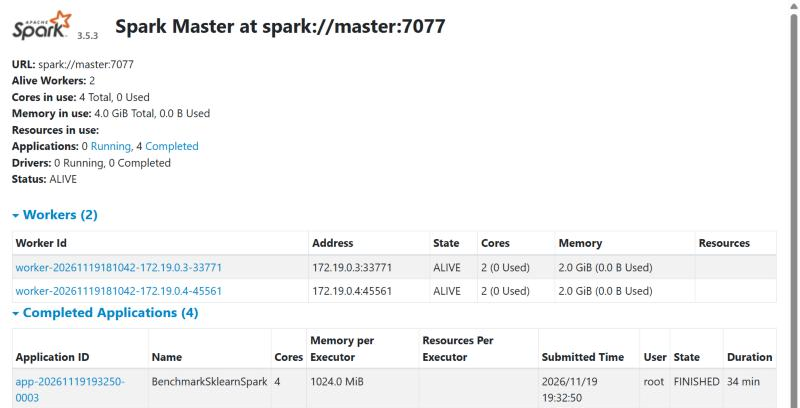
\includegraphics[width=\linewidth]{figures/spark_master_ui.png}
  \caption{Master : 2 workers vivants, 4 cœurs, application terminée.}
\end{subfigure}
\\[6pt]
\begin{subfigure}{0.56\textwidth}\centering
  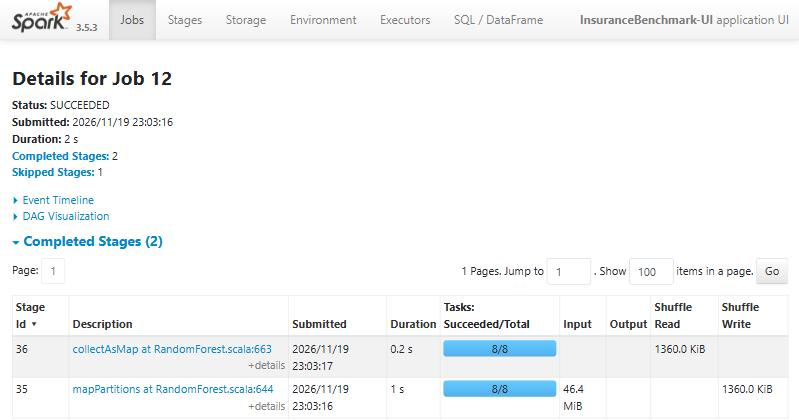
\includegraphics[width=\linewidth]{figures/spark_ui_stages_shuffle.png}
  \caption{Détail d'un job : 8 tâches par étape et shuffle écrit puis relu.}
\end{subfigure}\hfill
\begin{subfigure}{0.40\textwidth}\centering
  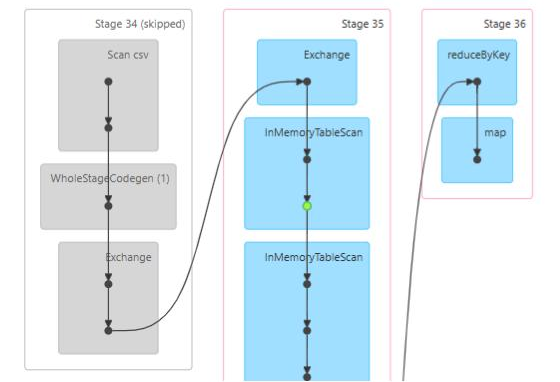
\includegraphics[width=\linewidth]{figures/spark_ui_dag.png}
  \caption{Graphe d'exécution (DAG) : une étape par cadre.}
\end{subfigure}
\caption{Captures des interfaces web de Spark.}
\label{fig:screens}
\end{figure}

% ================================================================== 6
\section{Résultats}

\subsection{Temps d'entraînement et seuil de basculement}

La figure~\ref{fig:fit} montre deux comportements très différents. La courbe de scikit-learn part de
quelques centièmes de seconde et croît à peu près comme le volume. Celles de Spark sont presque plates
sur les petits volumes : sur le jeu d'origine, la régression linéaire prend \spFitLRUn{}~s avec Spark
contre \skFitLRUn{}~s avec scikit-learn, environ \ratioLRUn{} fois plus. Ce plancher d'environ deux
secondes est le coût fixe de Spark : planification des jobs, lancement des tâches, échanges entre la
JVM et Python.

\begin{figure}[H]
\centering
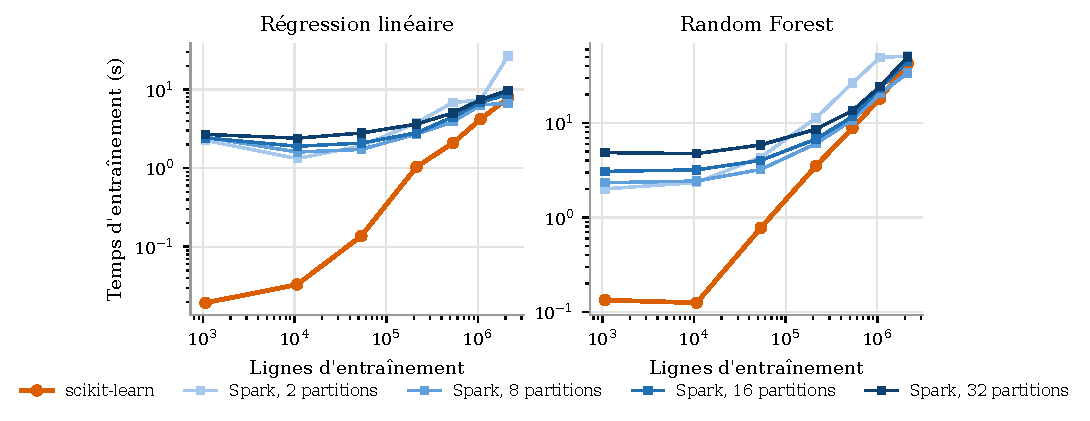
\includegraphics[width=\textwidth]{figures/fit_vs_volume.pdf}
\caption{Temps d'entraînement selon le volume, scikit-learn et Spark \code{local[*]} (échelles
logarithmiques).}
\label{fig:fit}
\end{figure}

\begin{table}[H]
\centering
\caption{Temps d'entraînement médians (s). Entre parenthèses : partitions de la meilleure exécution
Spark. Rapport = Spark / scikit-learn ; en gras, Spark plus rapide.}
\label{tab:fit}
\small
\begin{tabular}{l r r r r r r r}
\toprule
 & & \multicolumn{3}{c}{Régression linéaire} & \multicolumn{3}{c}{Random Forest} \\
\cmidrule(lr){3-5}\cmidrule(lr){6-8}
Volume & Lignes & sklearn & Spark & rapport & sklearn & Spark & rapport \\
\midrule
\inputtable{table_fit.tex}
\bottomrule
\end{tabular}
\end{table}

Le rapport entre les deux temps diminue régulièrement (tableau~\ref{tab:fit}, figure~\ref{fig:ratio}).
À \lin1000 (\nMilleTrain{} lignes), Spark est encore \ratioLRMille{} fois plus lent pour la régression
linéaire et \ratioRFMille{} fois pour la forêt. À \lin\scaleMax{} (\nMaxTrain{} lignes), la situation
s'inverse : \spFitLRMax{}~s contre \skFitLRMax{}~s pour la régression linéaire, \spFitRFMax{}~s contre
\skFitRFMax{}~s pour la forêt, soit des gains de \gainLRMax{} et \gainRFMax{}. Sur notre machine, le
seuil de basculement se situe donc \textbf{entre un et deux millions de lignes d'entraînement}, pour
les deux modèles ; les deux points qui l'encadrent ont été mesurés.

\begin{figure}[H]
\centering
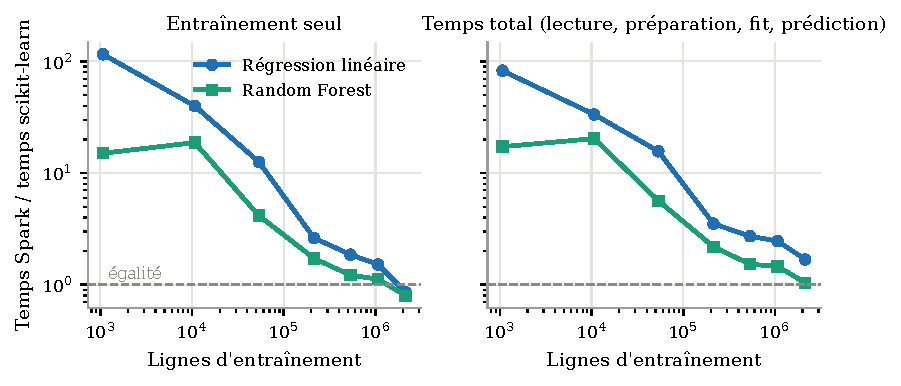
\includegraphics[width=\textwidth]{figures/ratio_basculement.pdf}
\caption{Temps Spark (meilleure configuration) divisé par le temps scikit-learn. Sous la ligne
pointillée, Spark est plus rapide.}
\label{fig:ratio}
\end{figure}

Le panneau de droite apporte une nuance. En temps total, Spark reste plus lent au plus grand volume :
\spTotLRMax{}~s contre \skTotLRMax{}~s pour la régression linéaire (rapport \ratioTotLRMax{}),
\spTotRFMax{}~s contre \skTotRFMax{}~s pour la forêt (rapport \ratioTotRFMax{}). Lire un CSV avec
Spark, le répartir et le mettre en cache coûte plus cher que de le lire avec pandas, et ce surcoût
n'est pas encore compensé à ce volume.

\subsection{Impact du nombre de partitions}

Les deux extrémités de la grille s'opposent (figure~\ref{fig:partitions}). Sur le jeu d'origine,
augmenter le nombre de partitions ne fait que ralentir : de 2 à 32 partitions, l'entraînement
s'allonge de \slowdownSmall\,\% en moyenne, car il n'y a presque rien à calculer et chaque partition
ajoute une tâche et des résultats à échanger. Au plus grand volume, 2 partitions deviennent au
contraire le pire réglage : la régression linéaire prend \spFitLRMaxPDeux{}~s contre \spFitLRMaxPHuit{}~s
avec 8 partitions, puisque deux tâches n'occupent que deux cœurs sur huit. Au-delà de 8, le temps
remonte (\spFitRFMaxPSeize{}~s puis \spFitRFMaxPTrenteDeux{}~s pour la forêt). Sur nos volumes, le
meilleur réglage est donc d'environ une partition par cœur. La documentation de Spark conseille
plutôt deux à trois tâches par cœur pour de gros traitements, ce qui laisse penser que l'optimum se
déplacerait sur des données nettement plus volumineuses.

\begin{figure}[H]
\centering
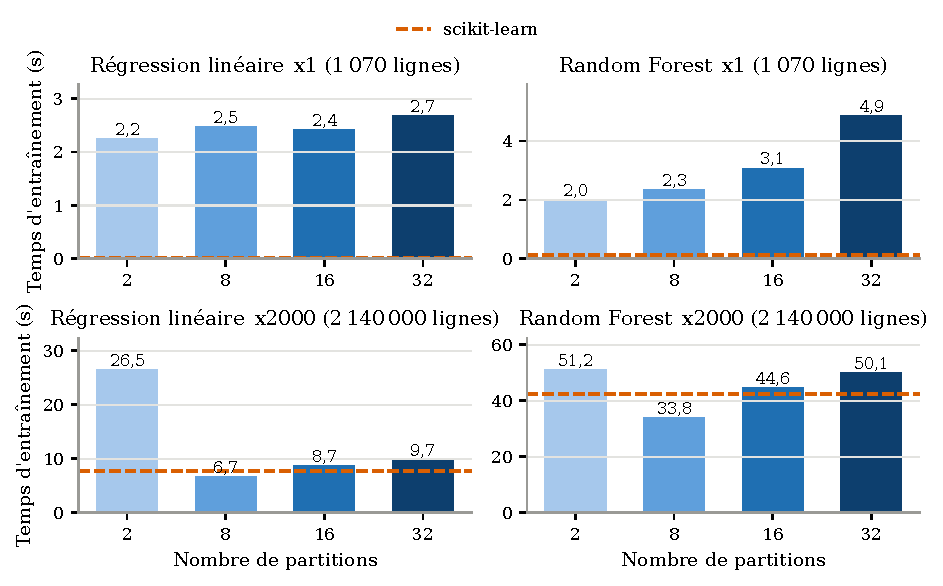
\includegraphics[width=0.94\textwidth]{figures/partitions.pdf}
\caption{Temps d'entraînement selon le nombre de partitions, au volume \lin1 (haut) et
\lin\scaleMax{} (bas).}
\label{fig:partitions}
\end{figure}

\subsection{Shuffle et mémoire}

Pour la forêt aléatoire, le shuffle croît avec le nombre de partitions (figure~\ref{fig:shufmem}) :
au volume \lin\scaleMax{}, il passe de \shufMaxRFPDeux{}~Mo avec 2 partitions à
\shufMaxRFPTrenteDeux{}~Mo avec 32, conséquence directe de l'agrégation des histogrammes. Pour la
régression linéaire, il reste à peu près constant (\shufMaxLRPDeux{} à \shufMaxLRPTrenteDeux{}~Mo) et
correspond surtout à la redistribution initiale des données. Côté mémoire, Spark part d'un plancher
d'environ \memSpMinUn{}~Go, la JVM réservant sa mémoire au démarrage, et atteint \memSpRFMax{}~Go au
plus grand volume contre \memSkRFMax{}~Go pour scikit-learn. La JVM étant réutilisée entre deux
exécutions, cette courbe se lit plutôt comme un maximum cumulé que comme une mesure isolée.

\begin{figure}[H]
\centering
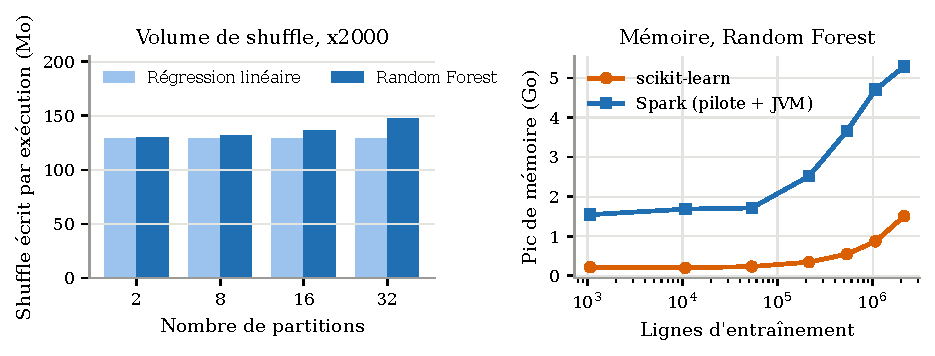
\includegraphics[width=\textwidth]{figures/shuffle_memoire.pdf}
\caption{À gauche : shuffle écrit par exécution (\lin\scaleMax{}). À droite : pic de mémoire de la
forêt aléatoire.}
\label{fig:shufmem}
\end{figure}

\subsection{Qualité des modèles}

Pour la régression linéaire, les deux bibliothèques obtiennent exactement le même résultat au plus
grand volume (R² de \rdeuxLRsk{}, RMSE de \rmseLRsk{}~\$). C'est attendu, le problème des moindres
carrés ayant une solution unique, et c'est la preuve que les deux frameworks sont évalués sur les
mêmes lignes. Pour la forêt aléatoire, scikit-learn fait un peu mieux (R² de \rdeuxRFsk{} contre
\rdeuxRFsp{}, RMSE de \rmseRFsk{} contre \rmseRFsp{}~\$). L'écart vient des algorithmes : pour
limiter les échanges, MLlib regroupe les variables continues en 32 intervalles (\code{maxBins}) avant
de chercher les seuils, alors que scikit-learn teste toutes les valeurs. Le choix de l'outil change
donc le coût bien plus que la qualité.

\subsection{Mode local et cluster}

Aucun basculement n'apparaît sur le cluster jusqu'à \lin\scaleCluMax{} (figure~\ref{fig:cluster}) :
Spark y reste \cCluSkRF{} fois plus lent que scikit-learn pour la forêt et \cCluSkLR{} fois pour la
régression linéaire. Il est aussi plus lent que le mode local, de \cCluLocalPctLR\,\% et
\cCluLocalPctRF\,\% respectivement. Le cluster ne dispose que de 4 cœurs contre 8, et ses exécuteurs,
désormais séparés, échangent leurs données par le réseau Docker au lieu de la mémoire d'un même
processus. Sur les petits volumes, les écarts entre les deux modes sont de quelques dixièmes de
seconde, du même ordre que la variabilité des mesures.

\begin{figure}[H]
\centering
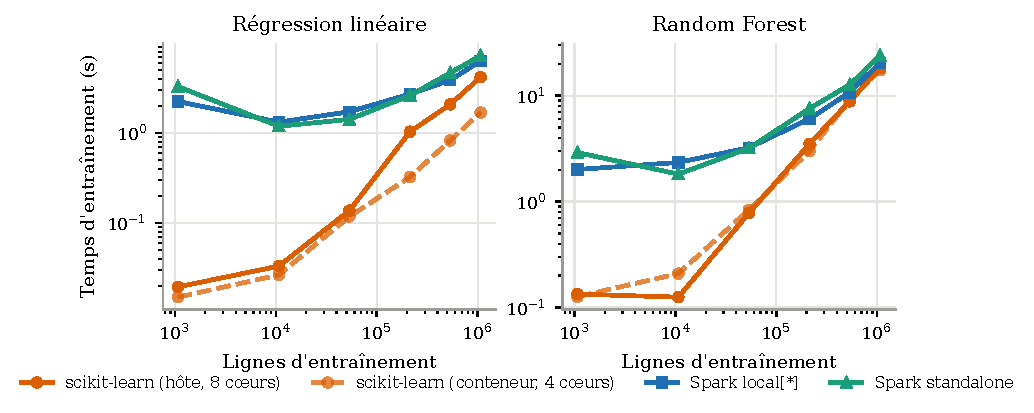
\includegraphics[width=\textwidth]{figures/local_vs_cluster.pdf}
\caption{Temps d'entraînement en mode local et sur le cluster \emph{standalone}.}
\label{fig:cluster}
\end{figure}

% ================================================================== 7
\section{Discussion}

Ces résultats s'expliquent par une décomposition simple du temps de Spark : un coût fixe, à peu près
indépendant du volume, plus un coût variable que le parallélisme permet de diviser. Tant que le
travail utile est faible, le coût fixe domine et scikit-learn l'emporte largement ; quand le volume
augmente, les huit cœurs de Spark finissent par rattraper puis dépasser scikit-learn. Le seuil est
approché plus tôt pour la forêt aléatoire : plus un modèle demande de calcul par ligne, plus le
parallélisme a de matière à répartir. L'expérience sur le cluster montre aussi que distribuer n'est
pas, en soi, accélérer : répartir le travail entre exécuteurs d'une même machine ajoute des échanges
sans ajouter de puissance. Le calcul distribué devient intéressant quand il donne accès à plus de
ressources qu'une machine n'en possède, en particulier quand les données ne tiennent plus en mémoire.

Plusieurs limites encadrent ces conclusions :
\begin{itemize}
  \item \textbf{une seule machine physique} : le cluster Docker est un vrai ordonnanceur Spark, mais il
        ne mesure pas le coût d'un réseau entre machines distantes ;
  \item \textbf{des données synthétiques}, qui mesurent la charge de calcul et non la qualité sur une
        population réelle plus grande ;
  \item \textbf{une mémoire partielle} : seuls le pilote et ses processus enfants sont mesurés, sans
        les exécuteurs distants du cluster ;
  \item \textbf{des environnements différents} (Windows et Python 3.11 en local, conteneurs Linux et
        Python 3.8 pour le cluster), d'où une comparaison des moteurs au sein de chaque environnement ;
  \item \textbf{un seuil propre au matériel}, qui se déplacerait sur une machine plus ou moins
        puissante, même si la méthode reste valable.
\end{itemize}

% ================================================================== 8
\section{Conclusion}

Nous avons construit un pipeline de régression identique avec scikit-learn et PySpark MLlib, et un
benchmark automatique qui fait varier le volume, le modèle et le partitionnement. Sur une seule
machine, scikit-learn est de loin le meilleur choix pour des volumes modestes : le coût fixe de Spark,
de l'ordre de deux secondes, dépasse largement le calcul utile. L'entraînement Spark devient plus
rapide entre un et deux millions de lignes, avec un gain de \gainLRMax{} à \gainRFMax{} au plus grand
volume testé, mais Spark n'a pas encore rattrapé scikit-learn en temps total. Le nombre de partitions
compte autant que le choix de l'outil, l'optimum étant ici d'environ une partition par cœur. Enfin,
le cluster \emph{standalone} monté sous Docker a confirmé que distribuer sur une même machine
physique ne fait qu'ajouter des échanges.

Le prolongement le plus naturel serait de refaire l'expérience sur au moins deux machines réelles
reliées en réseau local, afin de mesurer le coût des échanges entre machines ; la procédure est déjà
décrite dans le dépôt (\code{CLUSTER.md}). Il serait aussi utile de mesurer la mémoire des exécuteurs
et de travailler sur un jeu réellement volumineux, qui ne tienne pas en mémoire : c'est là que
scikit-learn atteint ses limites et que Spark trouve tout son intérêt. Tout le code et les résultats
bruts sont disponibles dans le dépôt du projet, et le benchmark se relance avec
\code{python benchmark\_sklearn\_spark.py}.

\end{document}
